\documentclass[11pt]{article}

% useful packages
\usepackage[english]{babel}
\usepackage{amsmath}
\usepackage{amssymb}
\usepackage{wasysym}
\usepackage{mathtools}
\usepackage{floatpag}
\usepackage{cite}
\usepackage{hyperref}
\usepackage{verbatim}
\usepackage{listings}
\usepackage{xcolor}
\usepackage{graphicx}
\usepackage{caption}
\usepackage{mwe}
\usepackage{float}


% colorful listings

\lstset{language=C,%
    breaklines=true,
    keywordstyle=\color{blue},
    morekeywords=[2]{1}, keywordstyle=[2]{\color{black}},
    identifierstyle=\color{black},%
    stringstyle=\color{olive},
    commentstyle=\color{gray},%
    showstringspaces=false,%without this there will be a symbol in the places where there is a space
    numbers=left,
    numberstyle={\tiny \color{black}},% size of the numbers
    numbersep=9pt, % this defines how far the numbers are from the text
    emph=[1]{for,end,break,if},emphstyle=[1]\color{red}, %some words to emphasise
}




\begin{document}

\title{Solution to Homework 4}

\author{
   Meshach Aruoriwo Ogbor,\\
   Md Rasel}

\maketitle

\section{Exercise 4.1 - Lattice Walk}
\lstinputlisting[language=C]{ex4_1.c}
%For compilation we use gcc 11.4 and openMPI 4.1.2. We compile with\\
%\verb+ mpicc -o hello_mpi hello_mpi.c+
For compilation on Stromboli, we used the following command: \\
\verb+ mpicc -o ex4_1 ex4_1.c+
\newpage

\section{Submit Script for exercise 4.1}
\lstinputlisting[language=bash]{job_ex4.sh}
\section{Results}
\verbatiminput{output.txt}
%Our main findings are summarized by fig.~\ref{fig1}.
We have faced some difficulties while reading the $\verb+directions.dat+$ file. At first, we tried without $\verb+ #define MAX_DIRECTIONS 1000+ $ and we got the final value but the program continued to run for an infinite time. Due to that we defined this and it successfully ended the program. If there is any better way, we would be open for your suggestions/recommendations.
\begin{figure} [H]
   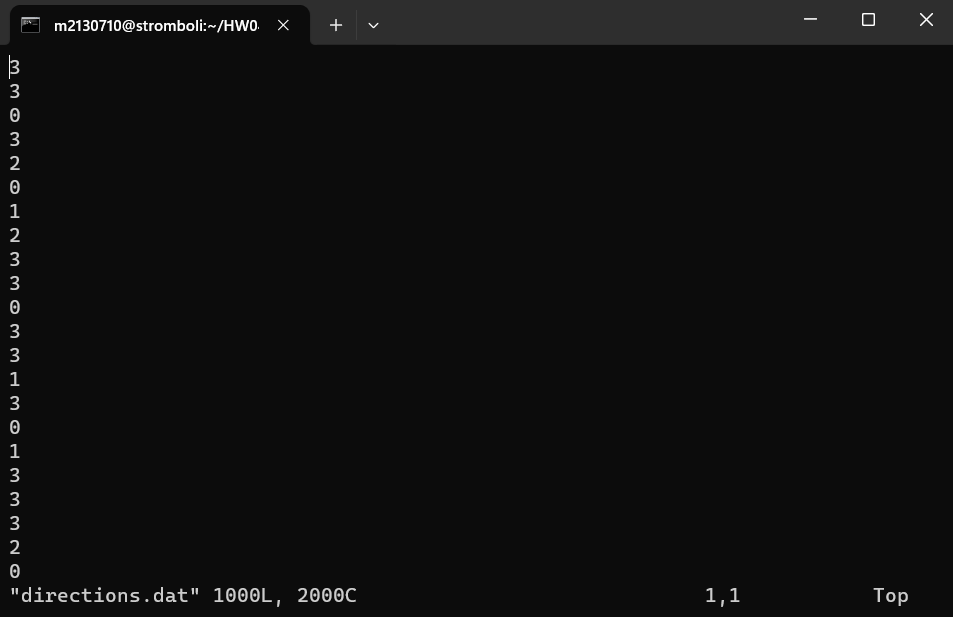
\includegraphics[width=\linewidth]{direction_file.png}
   %\caption{Skill level over time}\label{fig1}
\end{figure}

%\newpage
%\section{Exercise 3.2 - Tree}
%\lstinputlisting[language=C]{ex3_2.c}
%%For compilation we use gcc 11.4 and openMPI 4.1.2. We compile with\\
%%\verb+ mpicc -o hello_mpi hello_mpi.c+
%For compilation on Stromboli, we used the following command: \\
%\verb+ mpicc -o ex3_2 ex3_2.c -lm+ 
%\newpage
%
%\section{Submit Script for exercise 3.2}
%\lstinputlisting[language=bash]{job3_2.sh}
%\section{Results}
%\verbatiminput{output3_2.txt}
%As you can see from the results, time taken by the custom ``Tree'' function is less than the custom ``Loop'' function. For example: on rank 0, it took around 4 times less time (0.123695/0.032437) while using the ``Tree'' function. Theoretically, we should get $\log_2 48 = 5.5$ times less time. 
\end{document}
